\documentclass[t,compress,10pt,xcolor=dvipsnames]{beamer}

\usepackage{amsmath}
\newtheorem{mydef}{Definici\'on}
\usepackage{lmodern}
\usepackage[labelformat=empty,labelsep=none]{subfig}
\usepackage{caption}
\usepackage{float}
\usepackage{wrapfig}

\newcommand*\oldmacro{}%
\let\oldmacro\insertshorttitle% 
\renewcommand*\insertshorttitle{%
\oldmacro\hfill%
\insertframenumber\,/\,\inserttotalframenumber}

\definecolor{UniDunkel}{RGB}{73,142,137}
\definecolor{UniHell}{RGB}{142,184,182}

\setbeamertemplate{blocks}[rounded][shadow=true]
\setbeamercolor{structure}{fg=UniDunkel}

\setbeamercolor{block body}{parent=normal text,use=block title,bg=block title.bg!10!bg}
\setbeamercolor{block body alerted}{parent=normal text,use=block title alerted,bg=block title alerted.bg!10!bg}
\setbeamercolor{block body example}{parent=normal text,use=block title example,bg=block title example.bg!10!bg}

\setbeamercolor*{palette primary}{use=structure,fg=white,bg=UniDunkel!115}
\setbeamercolor*{palette secondary}{use=structure, fg=UniHell,  bg=UniHell}
\setbeamercolor*{palette tertiary}{use=structure,fg=white,bg=UniDunkel!115}
\setbeamercolor*{palette quaternary}{fg=Orange}

\setbeamercolor*{sidebar}{use=structure,bg=structure.fg}
\setbeamercolor*{palette sidebar primary}{use=structure,fg=structure.fg!10}
\setbeamercolor*{palette sidebar secondary}{fg=white}
\setbeamercolor*{palette sidebar quaternary}{fg=white}
\setbeamercolor*{titlelike}{parent=palette primary}

\setbeamercolor*{fine separation line}{}

\setbeamercolor{block title}{use=structure,fg=white,bg=structure.fg!0!red}
\setbeamercolor{block title alerted}{use=alerted text,fg=white,bg=alerted text.fg!0!white}
\setbeamercolor{block title example}{use=example text,fg=white,bg=example text.fg!0!white}

\useoutertheme{miniframes}
\useinnertheme{circles}
\setbeamertemplate{footline}[frame number]

\beamertemplatenavigationsymbolsempty

\usepackage{textpos} 
\usepackage{mathptmx}
\usepackage{anyfontsize}
\usepackage{t1enc}
\usepackage{multicol}
\usepackage{lmodern}

%\addtobeamertemplate{frametitle}{}{%
%\begin{textblock*}{100mm}(11cm,-1cm)
%	\includegraphics[height=1cm]{logo.png}
%\end{textblock*}}

%\titlegraphic{
%	\includegraphics[width=5cm]{backg}
%}

\title{\textbf{Agrupamiento y clasificaci\'on en la recuperaci\'on de informaci\'on en la web}}

%\author{Integrantes:\\
%	Marcos Manuel Tirador del Riego\\ 
%	Laura Victoria Riera P\'erez\\
%	Leandro Rodr\'iguez Llosa}
%\institute{Ciencias de la computaci\'on}
\date{}

%\usepackage{tikz}
%\titlegraphic { 
%	\begin{tikzpicture}[remember picture]
%		\node[left=0.2cm] at (current page.30){
%			\includegraphics[width=10cm]{backg}
%		};
%	\end{tikzpicture}
%}

\setbeamercolor{block body}{bg=Emerald,fg=Emerald}



\begin{document}
	
	\begin{frame}
		\begin{center}
			\begin{block}{}
				\centering
				\Large\textcolor{white}{\textbf{Agrupamiento y clasificaci\'on en la recuperaci\'on de informaci\'on en la web}}
			\end{block}
		
		\vspace{0.5em}
		
\includegraphics[width=3cm]{clustering.jpg}
		
		\vspace{0.5em}
		\footnotesize
		Integrantes:\\
			Marcos Manuel Tirador del Riego\\ 
			Laura Victoria Riera P\'erez
		
		\vspace{0.7em}
		\tiny	
		Tercer año. Ciencias de la computaci\'on. Universidad de La Habana. Cuba.
		
		\vspace{0.7em}
		\scriptsize
		Noviembre, 2022
		\end{center}
	\end{frame}

	\begin{frame}[allowframebreaks]{\'Indice general}
		\tableofcontents[sections={1}]
		\framebreak
		\tableofcontents[sections={2-4}]
	\end{frame}

	\frame{
		\frametitle{Aprendizaje no supervisado vs. aprendizaje supervisado}
		\begin{center}
			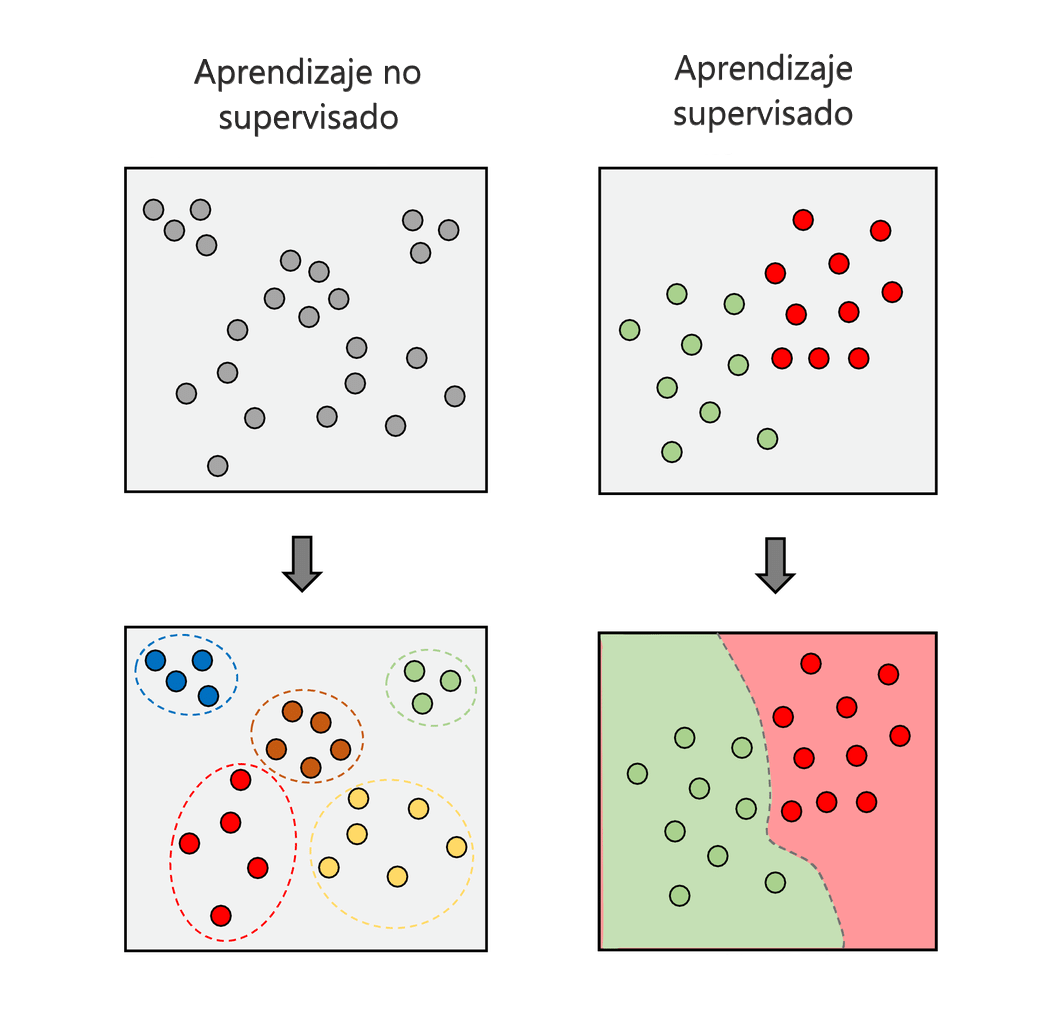
\includegraphics[width=7cm]{UL_vs_SL.png}
		\end{center}
	}
	\section{Agrupamiento}
	\frame[allowframebreaks]
	{
		\frametitle{Agrupamiento}
		\vspace{1em}
		Los algoritmos de agrupamiento conglomeran un conjunto de documentos en subconjuntos o cl\'usteres. Son utilizados para generar una estructura de categorías que se ajuste a un conjunto de observaciones. 
		
	\begin{center}
		\vspace{0.5em}
		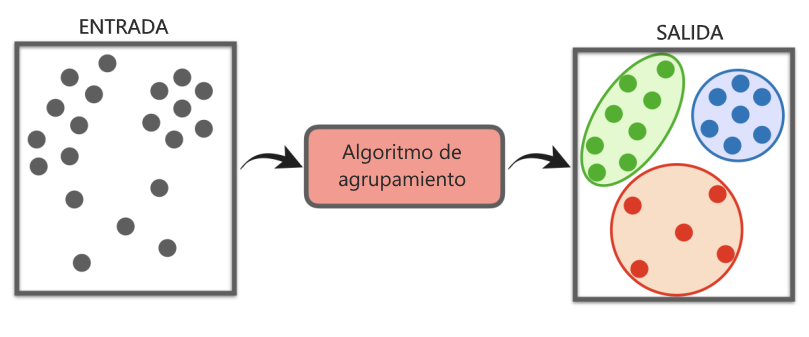
\includegraphics[width=10cm]{clustering_notion1.png}
	\end{center}
	}

	\frame{
		\frametitle{Caracter\'isticas generales}
		
		\vspace{4em}
		\begin{itemize}
			\item Es la forma más común de aprendizaje no supervisado.
			\item Los grupos formados deben tener un alto grado de asociación entre los documentos de un mismo grupo y un bajo grado entre miembros de diferentes grupos.
			\item La entrada clave para un algoritmo de agrupamiento es la medida de distancia. Diferentes medidas de distancia dan lugar a diferentes agrupamientos. 
		\end{itemize}
	}
	
	\frame{
		\frametitle{Hip\'otesis de agrupamiento}
		
		\vspace{5em}
		\textit{"Los documentos en el mismo grupo se comportan de manera similar con respecto a la relevancia para las necesidades de información."}
		
		\vspace{2em}
		La hipótesis establece que si hay un documento de un grupo que es relevante a una solicitud de búsqueda, entonces es probable que otros documentos del mismo clúster también sean relevantes. 
	}

	\frame{
		\frametitle{Clasificaci\'on de los algoritmos de agrupamiento}
		
		\vspace{2.5em}
		Seg\'un la pertenencia a los grupos:
		\begin{itemize}
			\item \textit{agrupamiento exclusivo o fuerte} (hard clustering): cada documento es miembro de exactamente un grupo.
			\item \textit{agrupamiento difuso o suave} (soft clustering): un documento tiene membresía fraccionaria en varios grupos.
		\end{itemize}
		
		\vspace{2em}
		Seg\'un el tipo de estructura impuesta sobre los datos:
		\begin{itemize}
			\item \textit{agrupamiento particionado o plano} (flat clustering)
			\item \textit{agrupamiento jer\'arquico} (hierarchical clustering).
		\end{itemize}
	}

	\subsection{Medidas de similitud entre documentos}
	\frame{
		\frametitle{Medidas de similitud}
		Sean $ d_{i} $ el $ i $-ésimo documento del corpus y $ w_{ik} $ el peso del t\'ermino $ k $ de un total $ N $ $ (N>0) $ en este documento.
		
		\begin{itemize}
			\vspace{0.5em}
			\item \textbf{Coeficiente de Dice:}
			\begin{center}
				$ S_{d_{i}, d_{j}} = \dfrac{2 \sum_{k=1}^{N} (w_{ik}w_{jk})}{\sum_{k=1}^{N}w_{ik}^{2} + \sum_{k=1}^{N}w_{jk}^{2}} $
			\end{center}
			
			\vspace{0.5em}
			\item \textbf{Coeficiente de Jaccard:}
			\begin{center}
				$ S_{d_{i}, d_{j}} = \dfrac{\sum_{k=1}^{N} (w_{ik}w_{jk})}{\sum_{k=1}^{N}w_{ik}^{2} + \sum_{k=1}^{max}w_{jk}^{2} - \sum_{k=1}^{N} (w_{ik}w_{jk})} $
			\end{center}
		
			\vspace{0.5em}
			\item \textbf{Coeficiente del coseno:}
			\begin{center}
				$ S_{d_{i}, d_{j}} = \dfrac{\sum_{k=1}^{N} (w_{ik}w_{jk})}{\sqrt{\sum_{k=1}^{N}w_{ik}^{2} \sum_{k=1}^{N}w_{jk}^{2}}} $
			\end{center}
		\end{itemize}
	
	}
	
	\subsection{Medidas de evaluaci\'on}
	\frame[allowframebreaks]
	{
		\frametitle{Medidas de evaluaci\'on}
		\begin{itemize}
			\vspace{5em}
			\item \textbf{Pureza}
			
			\item \textbf{Información mutua normalizada}
			
			\item \textbf{\'Indice de Rand (Rand Index)}
			
			\item \textbf{Medida F} 
		\end{itemize}	
	}

	\subsection{Agrupamiento particionado}
	\frame
	{
		\frametitle{Agrupamiento particionado}
		\vspace{7em}
		El agrupamiento particionado crea un conjunto  de clústeres sin ninguna estructura explícita que los relacione entre sí. 
	}
	
	\frame[allowframebreaks]
	{
		\frametitle{K-means}
		\vspace{3em}
		Es el algoritmo de agrupamiento particionado más importante. Su objetivo es minimizar la distancia euclidiana al cuadrado promedio entre los documentos y el centro de sus cl\'usteres. 
		
		El centro de un cl\'uster se define como la media o centroide $\mu$ de los documentos en un grupo $\omega$:
		
		\begin{center}
			$ \overrightarrow{\mu}(\omega) \leftarrow \dfrac{1}{|\omega_{k}|} \sum_{\overrightarrow{x} \in \omega_{k}} \overrightarrow{x} $
		\end{center}
		
		\framebreak
		\textcolor{white}{.}
		
		\vspace{2em}
		Una medida de qué tan bien los centroides representan a los miembros de su cl\'uster es la suma residual de cuadrados o RSS, que es la distancia al cuadrado de cada vector desde su centroide sumado sobre todos los vectores:
		
		\begin{center}
			$ RSS_{k} = \sum_{\overrightarrow{x} \in \omega_{k}}|\overrightarrow{x} - \overrightarrow{\mu}(\omega_{k})|^2$
			
			\vspace{1em}
			$ RSS = \sum_{k=1}^{K} RSS_{k} $
		\end{center}
		
		RSS es entonces la función objetivo en K-means y nuestro objetivo es minimizarla.
	
	\framebreak
	\textcolor{white}{.}
	
	\vspace{1em}
	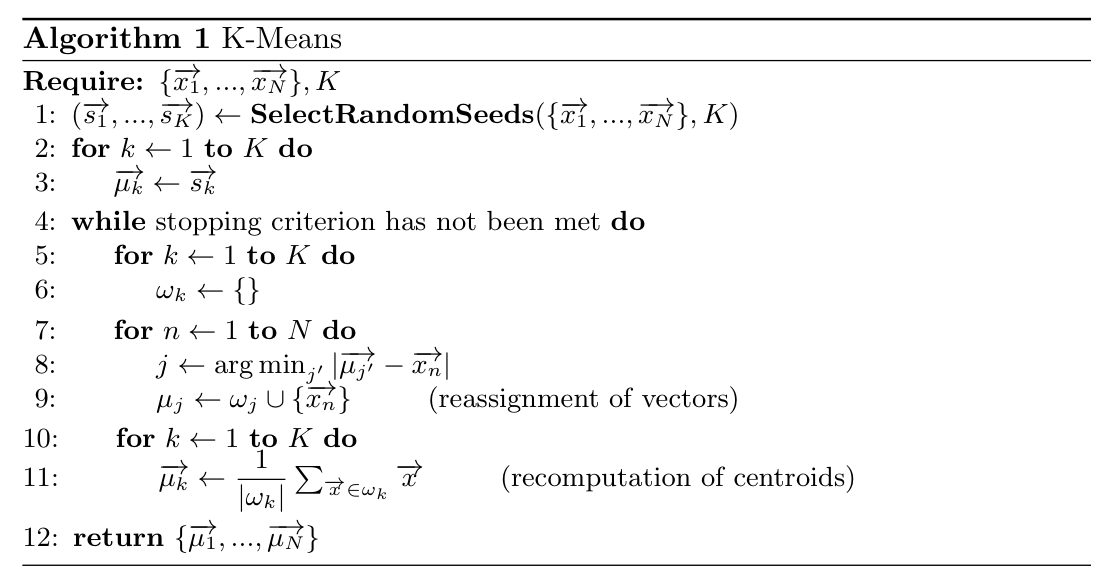
\includegraphics[width=10.5cm]{K-means.png}

	\framebreak
	
	\textcolor{white}{.}
	
	\vspace{0.5em}
	El primer paso de esta implementaci\'on de K-means es seleccionar al azar como centros iniciales de los cl\'usteres a K documentos, estas son las semillas. Luego, el algoritmo mueve los centros de los grupos en el espacio para minimizar el RSS. Este proceso se repite de manera iterativa hasta que se cumpla un criterio de parada.
	
	\vspace{1em}
	Criterios de parada:
	\begin{itemize}
		\item Cuando se ha completado un número fijo de iteraciones I. 
		\item Cuando la asignación de documentos a grupos no cambia entre iteraciones.
		\item Cuando los centroides no cambian entre iteraciones.
		\item Cuando RSS cae por debajo de un umbral.
	\end{itemize}
}

	\subsection{Agrupamiento jer\'arquico}
	\frame
	{
		\frametitle{Agrupamiento jer\'arquico}
		\vspace{2em}
		El agrupamiento jerárquico produce una jerarquía, una estructura que es más informativa que el conjunto no estructurado de clústeres devuelto por el agrupamiento particionado.
		
		\vspace{1em}
		Pueden tener dos enfoques: 
		\begin{itemize}
			\item De abajo hacia arriba (bottom-up) llamados de \textit{agrupamiento jer\'arquico aglomerativo}. 
			\item De arriba hacia abajo (top-down) conocidos como de \textit{agrupamiento jer\'arquico divisivo}. 
		\end{itemize}
	}
	
	
	\subsubsection{Agrupamiento jer\'arquico aglomerativo}
	\frame
	{
		\frametitle{Agrupamiento jer\'arquico aglomerativo}
		\vspace{3em}
		Los algoritmos de abajo hacia arriba tratan cada documento como un clúster único desde el principio y luego fusionan (o aglomeran) sucesivamente pares de grupos hasta que todos los grupos se han fusionado en uno solo que contiene todos los documentos. 
		Es por esto que se denomina agrupamiento jerárquico aglomerativo o HAC por sus siglas en ingl\'es. 
		
		\vspace{1em}
		Toman decisiones basadas en patrones locales sin tener inicialmente en cuenta la distribución global. Estas decisiones tempranas no se pueden deshacer.
	}

	\frame[allowframebreaks]
	{
		\frametitle{Medidas de similitud para cl\'usteres en HAC}
		
		\vspace{1em}
		\begin{itemize}
			\item \textbf{Agrupamiento por enlazamiento \'unico} (single link clustering): La similitud entre dos cl\'usters es la similitud de los dos objetos más cercanos entre ellos (mayor similitud).
	
			\item \textbf{Agrupamiento por enlazamiento completo} (complete link clustering): La similitud entre dos cl\'usters es la similitud de los dos objetos más alejados entre ellos (menor similitud). 
			
			\item \textbf{Agrupamiento aglomerativo por promedio de grupo} (group-average agglomerative clustering): Calcula la similitud promedio de todos los pares de documentos, incluidos los pares del mismo grupo, evitando así castigar valores extremos como en los criterios de enlace único y enlace completo.

			\item \textbf{Agrupamiento por centroide} (centroid clustering): La similitud de dos cl\'usters est\'a definida como la similitud de sus centroides.
		\end{itemize}
	
	}	
	
	\frame[allowframebreaks]
	{
		\frametitle{Algoritmo HAC}
		
		\vspace{1em}
		Dado un conjunto de N elementos a agrupar, el proceso básico del agrupamiento jerárquico aglomerativo es:
		\begin{enumerate}
			\item Se comienza con N cl\'usteres, resultado de asignar cada elemento al suyo propio. Se computa la matriz C de similitud de N×N.
			
			\item Se halla la similitud entre los pares de cl\'usteres con la medida deseada.
			
			\item Se toma el par más similar de clústeres y se combinan en un único clúster.
			
			\item Se calculan las similitudes entre el nuevo clúster y cada uno de los cl\'usteres antiguos.
			
			\item Se repiten los pasos 3 y 4 hasta que todos los elementos estén agrupados en un solo grupo de tamaño N.
		\end{enumerate}
	
	\framebreak
		\textcolor{white}{.}
	
	\vspace{0.9em}
	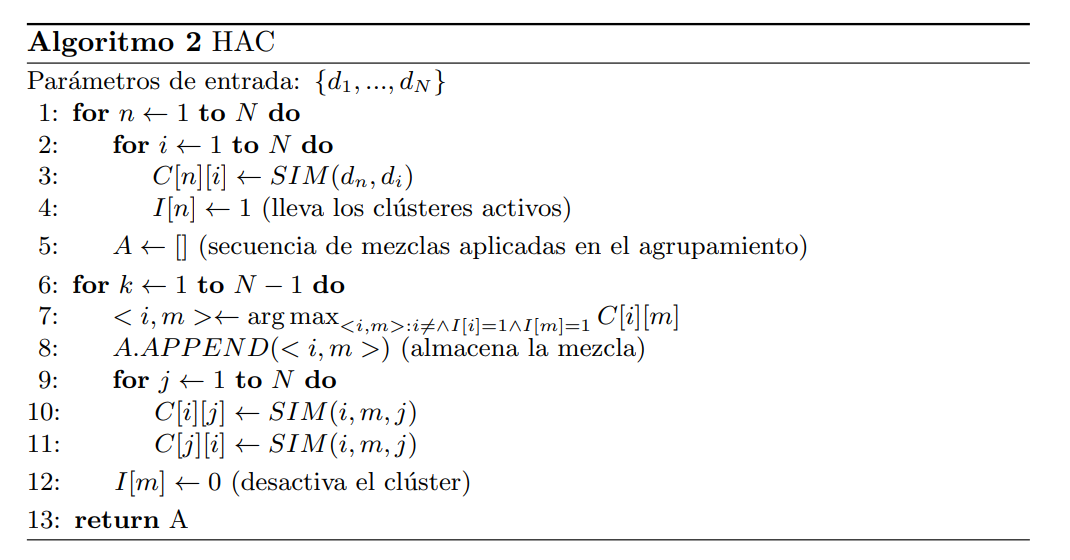
\includegraphics[width=10.5cm]{HAC.png}
	
	}	

	\subsubsection{Agrupamiento jer\'arquico divisivo}
	\frame
	{
		\vspace{4em}
		\frametitle{Agrupamiento jer\'arquico divisivo}
		Los algoritmos de arriba hacia abajo comienzan con todos los documentos en un grupo. El clúster se divide utilizando un algoritmo de agrupamiento particionado. Este procedimiento se aplica recursivamente hasta que cada documento está en su
		propio clúster.
		
		\vspace{0.5em}
		Se beneficia de la información completa sobre la distribución global al tomar decisiones de partición de alto nivel.
	}

	\subsection{Ventajas}
	\frame
	{
		\frametitle{Ventajas}
		\vspace{2.5em}
		\begin{itemize}
			\item No es necesario identificar las clases antes del procesamiento por lo que no se debe contar con expertos para este fin.
			
			\item Es útil para proporcionar estructura en grandes conjuntos de datos multivariados.
			
			\item Se ha descrito como una herramienta de descubrimiento porque tiene el potencial para revelar relaciones previamente no detectadas basadas en datos complejos.
			
			\item Debido a su amplia aplicación en dis\'imiles campos, cuenta el apoyo de una serie de paquetes de software, a menudo disponibles en la informática académica y otros entornos, por lo que se facilita su utilizaci\'on.
		\end{itemize}
	}

	\subsection{Desventajas}
	\frame
	{
		\frametitle{Desventajas}
		\vspace{6em}
		\begin{itemize}
			\item No se tiene una idea exacta de las clases creadas.
			\item No recibe retroalimentaci\'on.
		\end{itemize}
	}

	\subsection{Ejemplos de aplicaci\'on}
	\frame[allowframebreaks]
	{
		\frametitle{Ejemplos de aplicaci\'on en la web}
		\vspace{4em}
		El agrupamiento es una técnica importante para descubrir subregiones o subespacios relativamente densos de una distribución de datos multidimensional. Se ha utilizado en la recuperación de información para muchos propósitos diferentes, como la expansión de consultas, la agrupación e indexación de documentos y la visualización de resultados de búsqueda. Permiten mejorar interfaz y experiencia de usuario y proporcionar una mayor eficacia o eficiencia del sistema de búsqueda. 
		
		\framebreak
		\textcolor{white}{.}
		
		\vspace{2em}
		\begin{itemize}
			\item \textbf{Agrupamiento de resultados de búsqueda} (Search result clustering): La presentación predeterminada de los resultados de búsqueda (documentos devueltos en respuesta a una consulta) en la recuperación de información es una lista sencilla. Los usuarios escanean la lista de arriba a abajo hasta que encuentran la información que buscan. 
			
			En su lugar, en la agrupación en clústeres de resultados de búsqueda los documentos similares aparecen juntos, siendo más fácil escanear algunos grupos coherentes que muchos documentos individuales. Esto es particularmente útil si un término de búsqueda tiene diferentes significados.
			
			\framebreak
			\textcolor{white}{.}
			
			\vspace{1em}
			\item \textbf{Dispersión-recopilación} (Scatter-Gather): Su objetivo es tambi\'en una mejor interfaz de usuario. Este agrupa toda la colección para obtener grupos de documentos que el usuario puede seleccionar o reunir manualmente. Los grupos seleccionados se fusionan y el conjunto resultante se vuelve a agrupar. Este proceso se repite hasta que se encuentre un grupo de interés.
			
			La navegación basada en la agrupaci\'on de clústeres es una alternativa interesante a la búsqueda por palabras clave, el paradigma de recuperación de información estándar. Esto es especialmente cierto en escenarios donde los usuarios prefieren navegar en lugar de buscar porque no están seguros de qué términos utilizar en la búsqueda.
			
			\framebreak
			\textcolor{white}{.}
			
			\item \textbf{Recuperaci\'on basada en cl\'usteres} (Cluster-based retrieval): La búsqueda en el modelo de espacio vectorial equivale a encontrar los vecinos más cercanos a la consulta. El índice invertido admite la búsqueda rápida del vecino más cercano para la configuración, sin embargo, a veces es posible que no se pueda usar un índice invertido de manera eficiente. En tales casos, se podr\'ia calcular la similitud de la consulta con cada documento, pero esto es lento. 
			
			La hipótesis de agrupamiento ofrece una alternativa: encontrar los cl\'usteres que están más cerca de la consulta y sólo considerar los documentos de estos. Como hay muchos menos clústeres que documentos, se disminuye grandemente el espacio de b\'usqueda. Adem\'as, los elementos que coinciden con una consulta son similares entre sí, por lo que tienden a estar en los mismos cl\'usteres, de esta forma la calidad no disminuye en gran medida.
		\end{itemize}
	}

	\section{Clasificaci\'on}
	\frame[allowframebreaks]
	{
		\frametitle{Clasificaci\'on}
		\vspace{6em}
		El problema de clasificaci\'on en sentido general consiste en determinar dentro de un conjunto de clases a cu\'al de ellas pertenece un objeto dado. En el marco de este documento es de inter\'es estudiar la clasificaci\'on de textos. 
		
		La forma m\'as antigua de llevar a cabo la clasificaci\'on es manualmente. Por ejemplo, los bibliotecarios clasifican los libros de acuerdo a ciertos criterios, de modo que encontrar una informaci\'on buscada no resulte una tarea de gigante dificultad. Sin embargo, la clasificaci\'on manual tiene sus l\'imites de escalabilidad. 
		
		\framebreak
%		\textcolor{white}{.}
		
		Como alternativa podr\'ia pensarse el uso de \emph{reglas} para determinar autom\'aticamente si un texto pertenece o no a una clase determinada de documentos.
		
		Se ilustrar\'a un ejemplo de regla aplicada autom\'aticamente. Supongamos que un usuario necesita hacer una consulta en una p\'agina de noticias, por ejemplo, necesita tener actualidad sobre noticias relacionadas con las finanzas para tomar decisiones en su negocio. Al usuario entonces le podr\'ia interesar que de hacer una consulta en el sistema dicha consulta se mantenga ejecutando y le provea peri\'odicamente las noticias relativas a finanzas. 
		
		\framebreak
		
		A este tipo de consultas se le denomina consultas permanentes  (o \emph{standing querys} en ingl\'es). Una consulta permanente es aquella que se ejecuta peri\'odicamente en una colecci\'on a la cual nuevos  documentos se adicionan en el tiempo. Toda consulta permanente se puede ver como un tipo de regla que se aplica a un sistema de clasificaci\'on que divide una colecci\'on en documentos que satisfacen la consulta y documentos que no.
		
		
		%	 Por ejemplo las consultas permanentes son un ejemplo de regla aplicada autom\'aticamente. Una consulta permanente es como una consulta normal pero que es ejecutada repetidamente sobre una colecci\'on de textos a la cual se van adicionando documentos nuevos constantemente. Su finalidad es determinar si los nuevos textos pertenecen o no a la clase en cuesti\'on.
		
		Una regla captura una cierta combinaci\'on de palabras claves que identifican una clase. Reglas codificadas a mano pueden llegar a ser altamente escalable, pero crearlas y mantenerlas requiere un elevado costo en recursos humanos.
		
		\framebreak
		\textcolor{white}{.}
		
		Existe, sin embargo, un enfoque adicional a los dos anteriores mencionados. Este es el uso de \emph{Aprendizaje de M\'aquinas}. En este enfoque el conjunto de reglas de clasificaci\'on, o en general, el criterio usado para clasificar, es aprendido de forma autom\'atica a partir de los datos de entrenamiento.
		
		Al uso del Aprendizaje de M\'aquinas en la clasificaci\'on de textos se le conoce como clasificaci\'on estad\'istica de texto (o en ingl\'es \emph{statistical text classification}) si el m\'etodo de aprendizaje usado es estad\'itico.
		
		\framebreak
		
		Se presenta a continuaci\'on la definici\'on formal del problema de clasificaci\'on de textos, en el contexto del Aprendizaje de M\'aquinas.
		
		\vspace{.5em}
		
		\textbf{Definici\'on:}
			Sea $\mathcal{{X}}$ el espacio de documentos y $\mathcal{C} := \{c_i \mid c_i \subset \mathcal{X}, i \in \{ 1,2,\dots,n\} \}$ un conjunto fijo de clases (tambi\'en llamadas categor\'ias o etiquetas). Sea adem\'as $D$ un conjunto entrenado de documentos clasificados $(d,c) \in \mathcal X \times \mathcal{C}$. El \emph{problema de la clasificaci\'on de textos} consiste en encontrar, usando m\'etodos o algoritmos de aprendizaje, una funci\'on \emph{clasificadora} $\gamma : \mathcal{X} \rightarrow \mathcal{C}$, que mapee documentos a clases, que satisfaga que $D \subset \gamma$. 	
		
		\framebreak
		
		El aprendizaje que toma parte en la b\'usqueda de $\gamma$ es llamado \emph{aprendizaje supervisado} debido a que se necesita la ayuda de uno o varios expertos que creen el conjunto de entrenamiento $D$. Estos expertos son  tambi\'en quienes determinan el conjunto de clases en que se clasificar\'an los textos. Se denotar\'a  por $\Gamma$ el m\'etodo de aprendizaje supervisado descrito, el cual act\'ua como una funci\'on que mapea un conjunto de datos de entrenamiento en una funci\'on clasificadora, o sea que $\Gamma(D) = \gamma$.
		
		La definici\'on \ref{Problema_de_clasificacion} implica que cada documento pertenece a una sola clase. Pero existe otro tipo de problemas que permiten que un documento pertenezca a m\'as de una clase. Por ahora este trabajo se enfocar\'a en el tipo de una clase.
		
	
	}
	
	\subsection{Naive Bayes}
	\frame{
		\frametitle{Naive Bayes}
	}

	\subsection{Feature Selection}
	\frame{
		\frametitle{Feature Selection}
	}

	\subsection{K Nearest Neighbor}
	\frame{
		\frametitle{K Nearest Neighbor}
	}
	
	\subsection{Medidas de evaluaci\'on}
	\frame
	{
		\frametitle{Medidas de evaluaci\'on}	
	}
	
	\subsection{Ventajas}
	\frame
	{
		\frametitle{Ventajas}
	}
	
	\subsection{Desventajas}
	\frame
	{
		\frametitle{Desventajas}
	}
	
	\subsection{Aplicaciones en la Recuperaci\'on de la Informaci\'on}
	\frame
	{
		\frametitle{Aplicaciones en la Recuperaci\'on de la Informaci\'on}
	}
	
	\subsection{Otros ejemplos de aplicaci\'on}
	\frame
	{
		\frametitle{Otros ejemplos de aplicaci\'on}
	}

%	\section{Conclusiones}
%	\frame
%	{
%		\frametitle{Conclusiones}
%	}
%
%	\section{Referencias}
%	\frame
%	{
%		\frametitle{Referencias}
%	}
\end{document} 